% !TEX encoding = UTF-8
% !TEX TS-program = pdflatex
% !TEX root = ../tesi.tex

%**************************************************************
\chapter{Sviluppo Add-On}
\label{cap:sviluppo-addon}
%**************************************************************

\intro{In questo capitolo approfondiremo lo sviluppo dell'add-on}


\section{Analisi dei requisiti}
\subsection{Introduzione}

\begin{flushleft}
	\item Fulcro dell'attività di stage è stata la produzione e sviluppo di un add-on, un'applicazione a maschera, applicabile al client SAP.
	
	Lo scopo di quest'add-on è la stampa di un form o tabella di un modulo di SAP, ad esempio il form Scheda Attrezzatura, oppure l'esportazione su file esterno.
	\item Quest'applicazione è stata codificata in Microsoft Visual Studio, con le librerie di SAP Business One, in linguaggio C\#.
	
	Per realizzarlo c'è stato un periodo di formazione personale su il linguaggio C\# e sulle librerie di SAP per lo sviluppo degli add-on.
\end{flushleft}
\vspace{1em}


Continuiamo con la presentazione dei casi d'uso e il tracciamento dei requisiti.
\newpage

\subsection{Casi d'uso}
\begin{flushleft}
	Per lo studio dei casi di utilizzo del prodotto sono stati creati dei diagrammi.
	
	I diagrammi dei casi d'uso (in inglese \emph{Use Case Diagram}) sono diagrammi di tipo \gls{uml} dedicati alla descrizione delle funzioni o servizi offerti da un sistema, così come sono percepiti e utilizzati dagli attori che interagiscono col sistema stesso.
\end{flushleft}


\begin{figure}[!h] 
	\centering 
	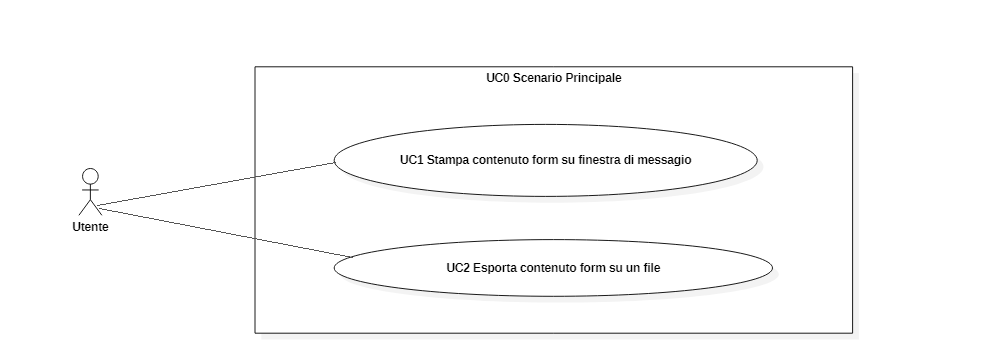
\includegraphics[scale = 0.4]{immagini/usecase/usecase-addon-uc0.png} 
	\caption{Use Case - UC0: Scenario principale}
\end{figure}
\begin{usecase}{0}{Scenario principale}
	\usecasepre{L'utente è entrato in un form del SAP}
	\usecasedesc{L'add-on mette a disposizione le funzionalità di stampa o salvataggio su file, dei contenuti del form}
	\usecasepost{Il sistema è pronto per permettere una nuova interazione}
	\label{uc:scenario-principale}
\end{usecase}
\begin{figure}[!h] 
	\centering 
	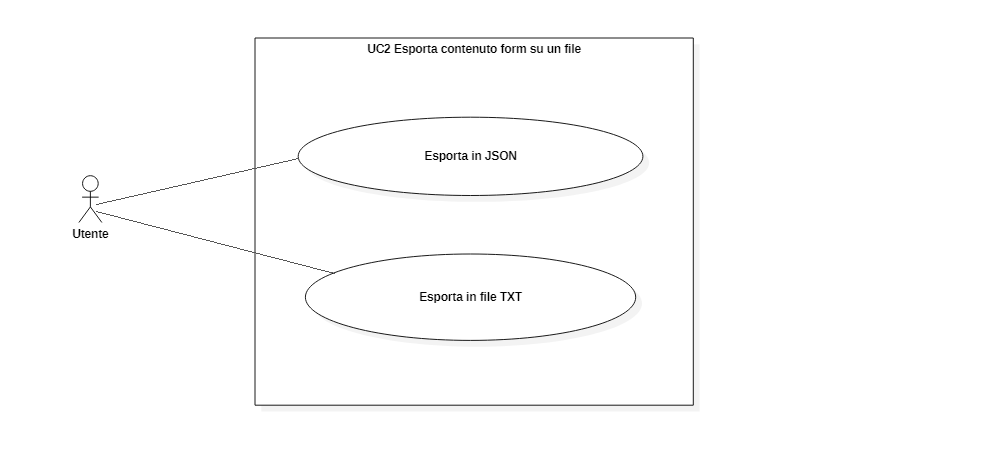
\includegraphics[scale = 0.4]{immagini/usecase/usecase-addon-uc2.png} 
	\caption{Use Case - UC2: Esporta contenuto form su un file}
\end{figure}
\begin{usecase}{2}{Esporta contenuto form su un file}
	\usecasepre{L'utente ha selezionato di salvare i contenuti del form su un file esterno}
	\usecasedesc{L'add-on metta a disposizione il salvataggio su file .txt o su file .json}
	\usecasepost{Il sistema è pronto per permettere una nuova interazione}
	\label{uc:esporta-file}
\end{usecase}

\newpage

\subsection{Tracciamento dei requisiti}
Da un'attenta analisi dei requisiti e degli use case effettuata sul progetto è stata stilata la tabella che traccia i requisiti in rapporto agli use case.

Sono stati individuati diversi tipi di requisiti e si è quindi fatto utilizzo di un codice identificativo per distinguerli.

Il codice dei requisiti è così strutturato R(F/Q/V)(N/D/O) dove:
\begin{enumerate}
	\item[R =] requisito
	\item[F =] funzionale
	\item[Q =] qualitativo
	\item[V =] di vincolo
	\item[O =] obbligatorio
	\item[D =] desiderabile
	\item[F =] facoltativo
\end{enumerate}
Nelle tabelle \ref{tab:requisiti-funzionali} e \ref{tab:requisiti-vincolo} sono riassunti i requisiti e il loro tracciamento con gli use case delineati in fase di analisi.


\begin{table}[!h]%
	\begin{tabularx}{\textwidth}{lXl}
		\hline\hline
		\textbf{Requisito} & \textbf{Descrizione} & \textbf{Use Case}\\
		\hline
		RFO-1     & L'add-on deve permettere di stampare il contenuto del form sotto forma di finestra di messaggio & UC1 \\
		RFO-2     & L'add-on deve permettere di esportare il contenuto del form in un file in formato JSON & UC2.1\\
		RFO-3     & L'add-on deve permettere di esportare il contenuto del form in un file in formato TXT & UC2.2\\
		\hline
	\end{tabularx}
	\caption{Tabella del tracciamento dei requisiti funzionali}
	\label{tab:requisiti-funzionali}
\end{table}%

\begin{table}[!h]%
	\begin{tabularx}{\textwidth}{lXl}
		\hline\hline
		\textbf{Requisito} & \textbf{Descrizione} & \textbf{Use Case}\\
		\hline
		RVO-1    & La versione di SAP Business One da utilizzare è la versione 10.0 & - \\
		\hline
	\end{tabularx}
	\caption{Tabella del tracciamento dei requisiti di vincolo}
	\label{tab:requisiti-vincolo}
\end{table}%

\newpage

\section{Realizzazione}
\begin{flushleft}
	Lo sviluppo dell'add-on è stato effettuato, come detto in precedenza, con linguaggio C\# e attraverso l'\gls{ide} Microsoft Visual Studio.
	
	Inoltre è stata usata una delle varie librerie fornite da SAP Business One SDK, ovvero:
	\begin{itemize}
		\item \textbf{SAPbouiCOM:} ovvero SAP Business One UI COM, una libreria COM di SAP Business One, per la gestione dell'interfaccia grafica(\emph{User Interface}).
	\end{itemize}
	Nella sezione precedente, non sono stati forniti diagrammi di classe poichè il codice dell'add-on, consiste in una classe che gestisce gli eventi generali ed una classe di supporto che gestisce gli eventi del form aperto.
	
	Dunque, essendo solo due classi, è stato ritenuto poco utile fornire diagrammi.
	
	\vspace{1em}
	Nel proseguo, viene illustrata una realizzazione tramite uno scenario di utilizzo.
\end{flushleft}
\begin{flushleft}
	Per prima cosa accediamo al SAP con le credenziali corrette ed entriamo su un form, di un modulo.
	
	In questo caso entriamo nel form Scheda Attrezzatura.
	
\end{flushleft}
\begin{figure}[!h] 
	\centering 
	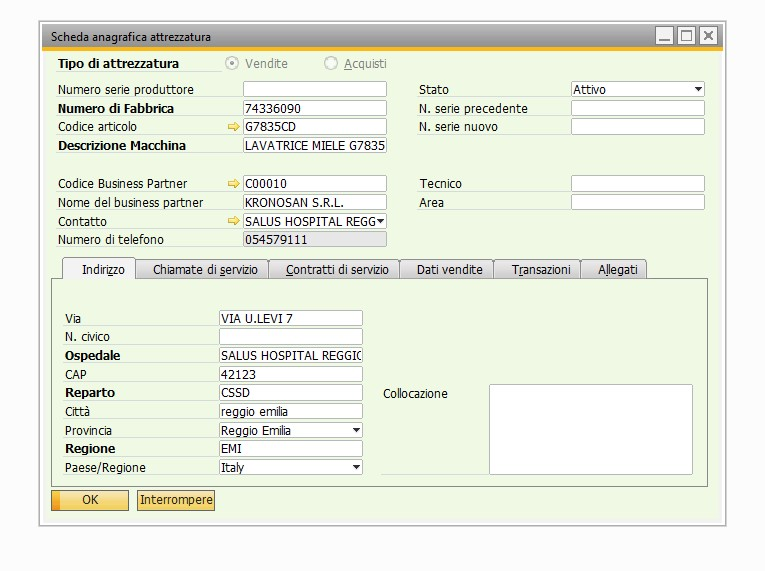
\includegraphics[scale = 0.6]{immagini/add-on/addon-scheda-nobutton.jpg} 
	\caption{Add-On, screenshot prima dell'attivazione dell'add-on}
\end{figure}
Come possiamo notare da questa figura abbiamo due pulsanti:
\begin{itemize}
	\item Ok;
	\item Interrompere.
\end{itemize}

\newpage

\begin{flushleft}
	Ora attiviamo l'add-on, per attivare l'add-on si può:
\end{flushleft}
\begin{itemize}
	\item installare l'addon nel client SAP locale;
	\item compilare e farlo eseguire su Microsoft Visual Studio, senza averlo installato nel client SAP;
	\item nel caso sia installato nel client SAP, si può impostare l'attivazione manuale o automatica;
	\item nel caso di attivazione manuale, bisogna andare sulle opzioni degli add-on installati ed attivarlo.
\end{itemize} 
\begin{flushleft}
	
	Una volta attivato l'add-on, riapriamo il modulo Scheda Attrezzatura e vedremo comparire un pulsante nuovo.
	
\end{flushleft}
\begin{figure}[!h] 
	\centering 
	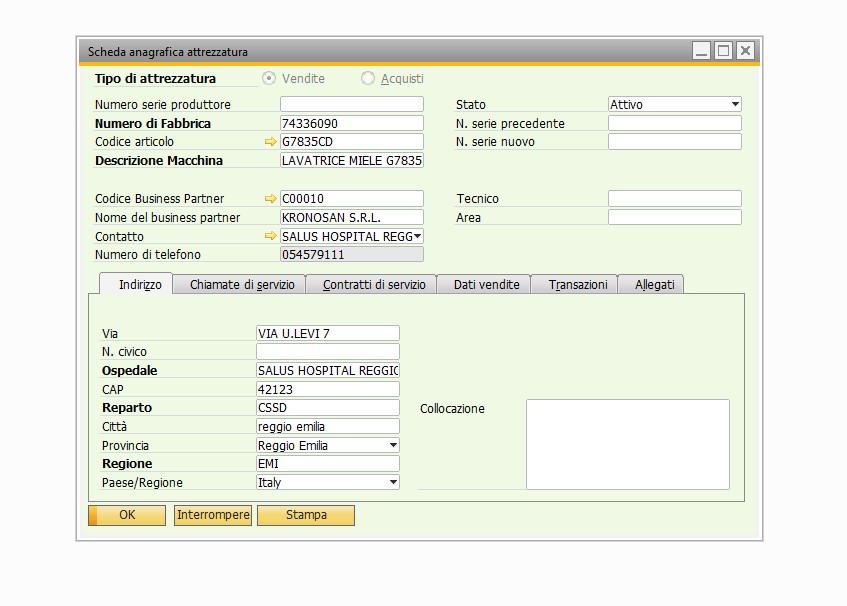
\includegraphics[scale = 0.6]{immagini/add-on/addon-scheda-yesbutton.jpg} 
	\caption{Add-On, screenshot dopo l'attivazione dell'add-on}
\end{figure}
\begin{flushleft}
	
	In questa figura è già stata selezionata un'attrezzatura, in questo caso l'ultima attrezzatura aggiunta nel database.
	
\end{flushleft}

\newpage

\vspace{1em}

Cliccando il pulsante Stampa si aprirà una nuova finestra.

\begin{figure}[!h] 
	\centering 
	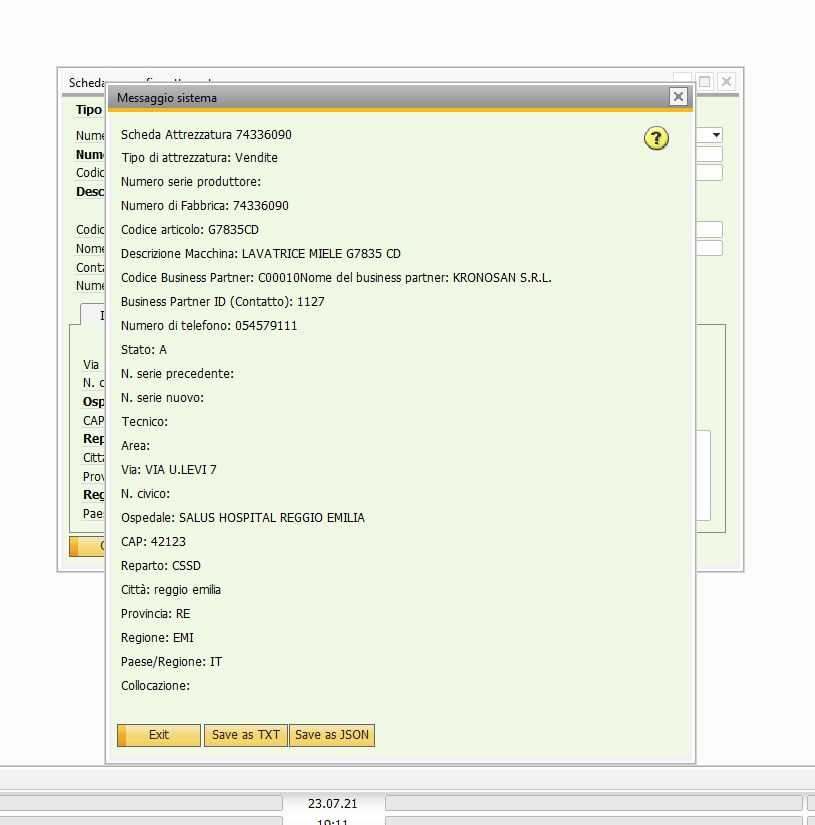
\includegraphics[scale = 0.6]{immagini/add-on/addon-stampa.jpg} 
	\caption{Add-On, stampa dei contenuti del form su finestra di messaggio}
\end{figure}
\begin{flushleft}
	
	Dopo aver cliccato il pulsante Stampa, si entra in questa finestra, dove abbiamo stampato su finestra di messaggio i contenuti del form; inoltre abbiamo altri 3 pulsanti:
\end{flushleft}
\begin{itemize}
	\item \textbf{Exit:} premendo questo pulsante, come dice il nome, usciremo da questa finestra;
	\item \textbf{Save as TXT:} premendo questo pulsante il contenuto di questa finestra verrà esportato su un file .txt, senza alcuna formattazione aggiuntiva;
	\item \textbf{Save as JSON:} premendo questo pulsante il contenuto di questa finestra verrà esportato su un file .json, con la formattazione json.
\end{itemize}

\begin{flushleft}
	Per come è ora programmato l'add-on, i file vengono salvati nella cartella dov'è installato l'add-on, in particolare vengono chiamati rispettivamente \textbf{file.txt} per il file TXT e \textbf{filejson.json} per il file JSON.
	
	Se questi file esistono già nella cartella, e viene premuto nuovamente il pulsante di salvataggio, i file verranno sovrascritti dall'ultimo file.
	
\end{flushleft}

\newpage

\begin{flushleft}
	
	Ora nei prossimi due screenshot, vedremo il contenuto dei due file, rispettivamente txt e json, esportati dall'add-on.
	
\end{flushleft}
\begin{figure}[!h] 
	\centering 
	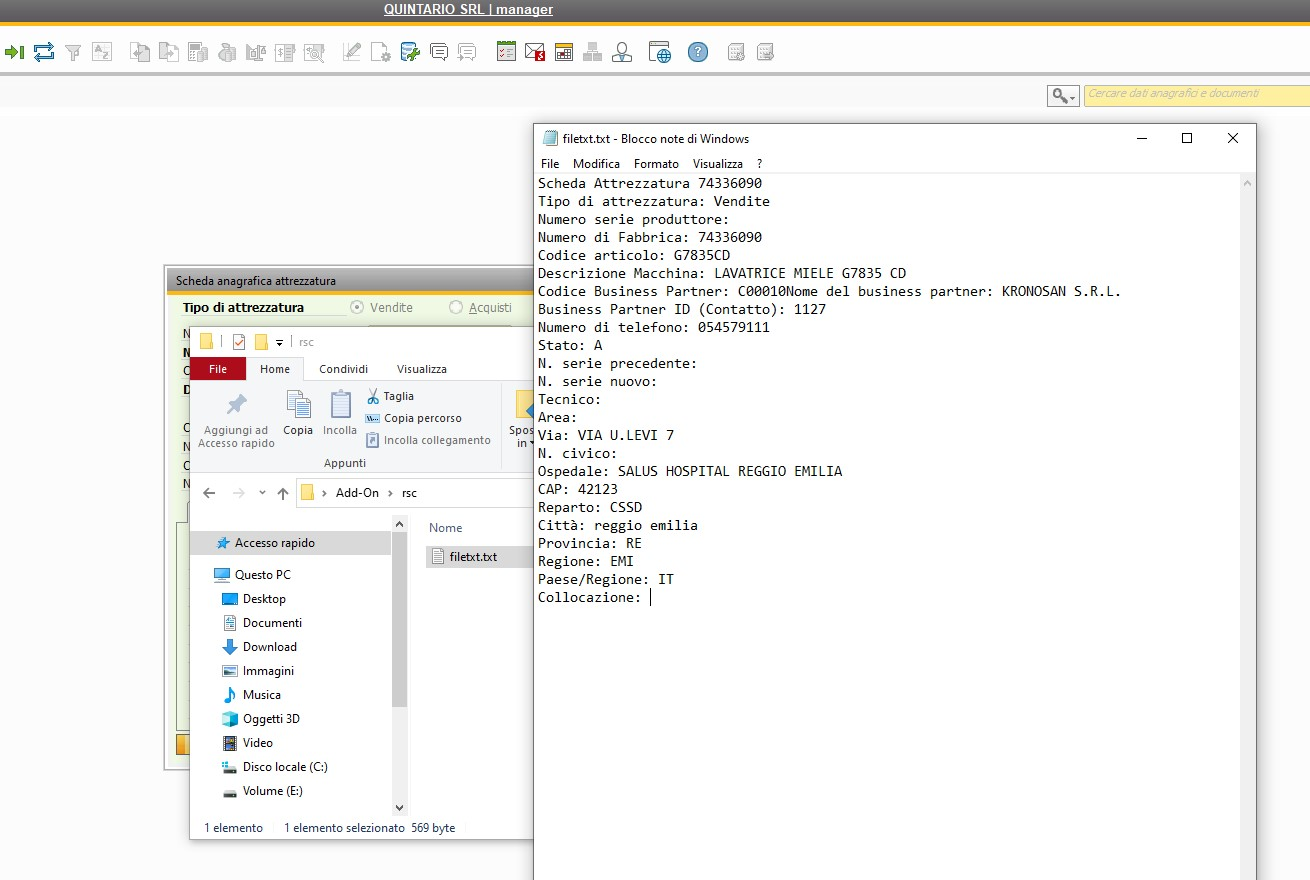
\includegraphics[scale = 0.38]{immagini/add-on/addon-esporta-txt.jpg} 
	\caption{Add-On, file txt esportato dall'add-on}
\end{figure}

\begin{figure}[!h] 
	\centering 
	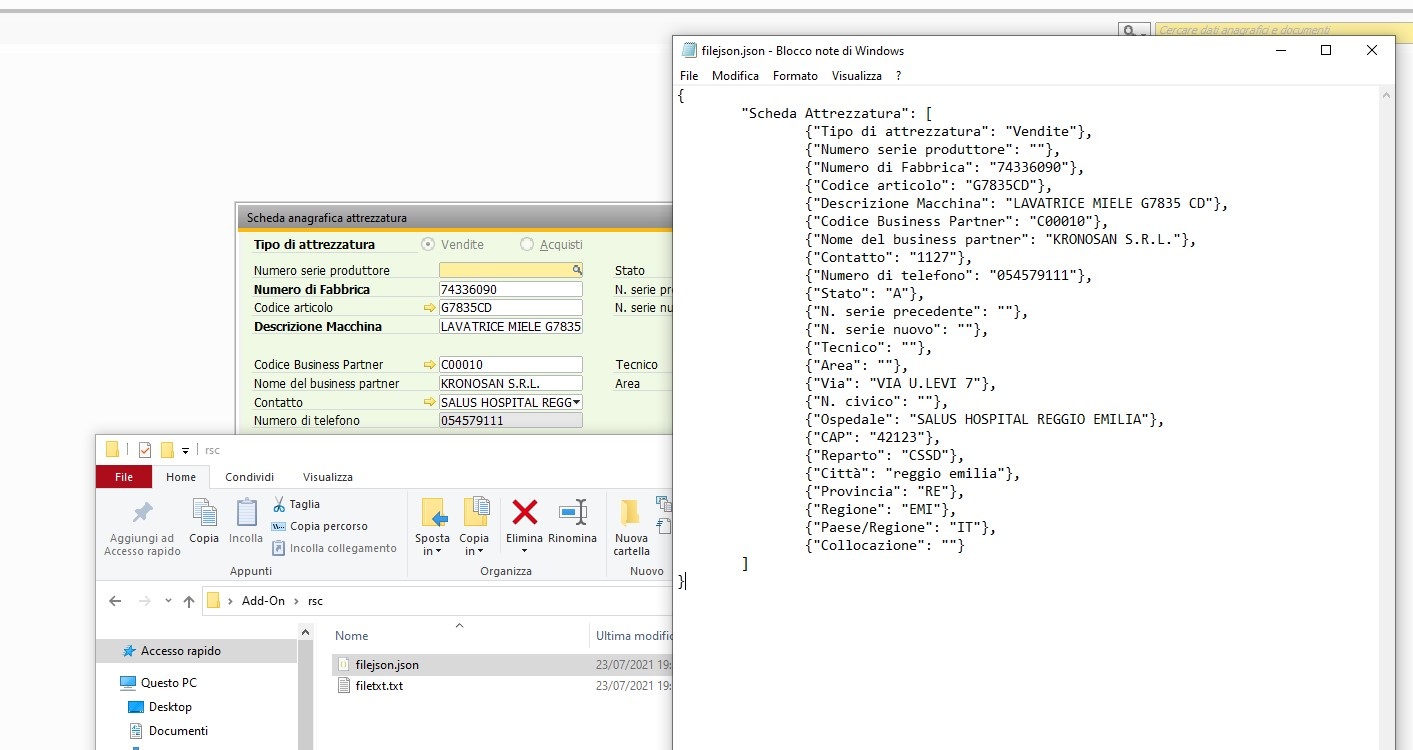
\includegraphics[scale = 0.38]{immagini/add-on/addon-esporta-json.jpg} 
	\caption{Add-On, file json esportato dall'add-on}
\end{figure}

\newpage

\section{Accettazione}
Riguardo la Verifica e Validazione, ovvero l'Accettazione, non abbiamo alcun test d'unità e test automatico.

Abbiamo invece una procedura per verificare il corretto funzionamento dell'applicazione, riportata qui vi seguito.

\begin{enumerate}
	\item Accedere al SAP Business One con le proprie credenziali;
	\item Attivare l'add-on dalle opzioni del client;
	\item Aprire il form Scheda Attrezzatura nel modulo dei Servizi;
	\item Selezionare un istanza di attrezzatura esistente, usualmente attraverso il numero di fabbrica, essendo chiave univoca di questa tabella;
	\item Cliccare il pulsante Stampa;
	\item Verificare che le informazioni stampate nella nuova finestra di messaggio apertasi corrispondano alle informazioni del form;
	\item Cliccare Save as JSON;
	\item Cliccare Save as TXT;
	\item Entrare nella cartella dell'add-on dove sono salvati i file;
	\item Verificare che il contenuto dei file corrisponda alle informazioni del form.
\end{enumerate}

Se non ci sono stati problemi in questi step, in particolare se le informazioni stampate nella finestra di messaggio e le informazioni salvate nei due file corrispondono alle informazioni presenti nel form Scheda anagrafica attrezzatura, l'add-on può considerarsi verificato e valido.

\subsection{Requisiti soddisfatti}
Logicamente i requisiti funzionali sono stati tutti soddisfatti, eccone qui una piccola tabella.

\begin{table}[!h]%
	\begin{tabularx}{\textwidth}{lXl}
		\hline\hline
		\textbf{Requisito} & \textbf{Descrizione} & \textbf{Use Case}\\
		\hline
		RFO-1     & Step 6 & Soddisfatto \\
		RFO-2     & Step 10 & Soddisfatto\\
		RFO-3     & Step 10 & Soddisfatto\\
		\hline
	\end{tabularx}
	\caption{Tabella del soddisfacimento dei requisiti funzionali}
	\label{tab:requisiti-funzionali-soddisfatti}
\end{table}%